\section{Introduction}
\begin{figure}
  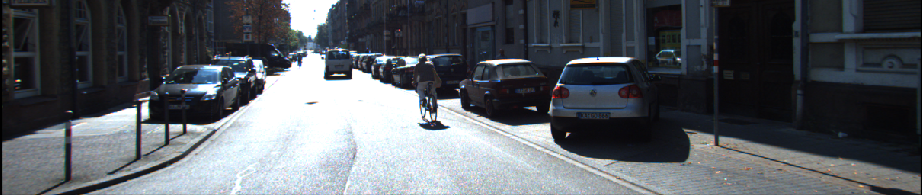
\includegraphics[width=0.6\textwidth]{intro-rgb}\\
  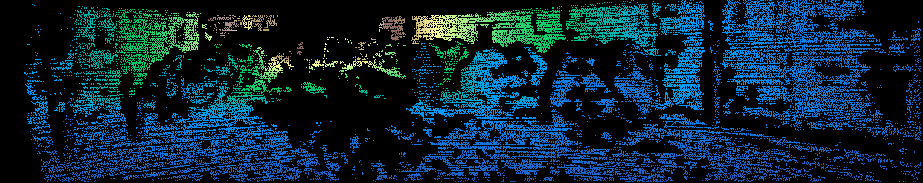
\includegraphics[width=0.6\textwidth]{intro-ground}\\
  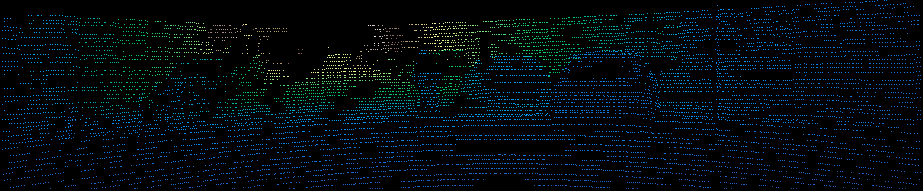
\includegraphics[width=0.6\textwidth]{intro-input}\\
  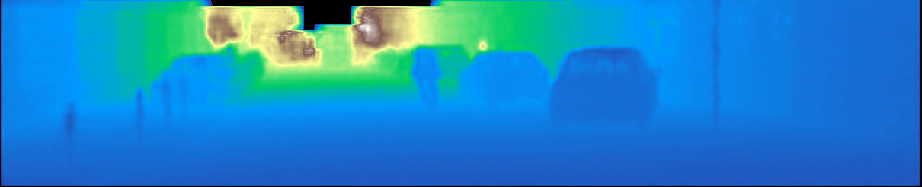
\includegraphics[width=0.6\textwidth]{intro-pred}
  \caption{From top to bottom: RGB image of scene, ground-truth depth, input to the network, our output. The bicycalist and bollards can barely be seen in the input map but a clearly represented in the output. Our method also accurately reconstructs very thin objects such as the sign post.}
  \label{fig:intro}
\end{figure}
In recent years 3D information has become an important component of robotic sensing. Usually this information is presented in 2.5D as a depth map, either measured directly using LIDAR or computed using stereo correspondence. Since LIDAR and stereo techniques yield few samples relative to modern image sensors, it has become desirable to convert sparse depth measurements into high resolution depth maps.


Recent works~\cite{} have directly applied deep networks to depth completion from sparse measures. However, common network architectures have two drawbacks when applied to this task: 1) They implicitly pose depth completion as finding a mapping from sparse depth maps to dense ones, instead of as finding a depth map that is consistent with the sparse input. This essentially throws away information and we observe that feed forward networks do not learn to propagate the input points through to the output. 2) Common networks are sensitive to the sparsity of the input since they treat all pixels equally, regardless of whether or not they represent samples or missing input. Special CNN networks have been designed to address this problem, but they still do not express the constraints given by the input~\cite{}. In this paper we address both of these issues with a novel deep recurrent autoencoder architecture which internally optimizes its depth prediction while respecting to both sparsity and input constraints.
%) Common networks are sensitive to the sparsity level of the input since they treat each pixel equally, regardless of whether it is an input or missing value. While special CNN architecture have been designed to achieve sparsity invariance~\cite{}, they have no way to handle the second issue. 2) Common networks do not explicitly enforce the constraint that the input depth map is a subset of the desired output. In fact, we observe that deep networks are not able to effectively propagate input depth samples to the output. In this paper we address both of these issues with a novel deep recurrent autoencoder architecture which internally optimizes its depth prediction while respecting to both sparsity and input constraints.


We have taken inspiration from Compressed sensing (CS), which provides a natural framework for this problem. Formally, CS is concerned with recovering signals from incomplete measurements by enforcing that signals be sparse when measured in an appropriate basis. This basis takes the form of an overcomplete dictionary matrix $A$ which maps sparse representations to observed signals.
% To reconstruct signals which are not measured, certain prior knowledge/assumption of the signal is required.

The choice of dictionary is crucial for recovering the signal efficiently, especially when the dimensionality is high. For high resolution imagery data, such as depth maps, multi-layer convolutional sparse coding~\cite{} is effective as it explicitly models local interactions through the convolution operator~\cite{} and captures higher level abstraction of the signal~\cite{} with tractable computational and model complexity. However, none of the existing multi-layer convolutional sparse coding algorithms are designed for data with large potion of missing values. This is reflected by the fact that recent works~\cite{} applying CS to depth completion are restricted to using single-level, hand crafted dictionaries. CS has also fallen out of fashion since the existing algorithms have difficult to interpret hyper-parameters, and often do not achieve good performance without careful tuning of these parameters.

% extracting sparse codes $x$ but learning an appropriate $A$ from data proves challenging, especially with a large amount of data or large dimensionality. Learning dictionaries is especially difficult in layered sparse coding where one seeks a very high level sparse representation $x_{\ell}$ such that $b = A_0A_1\ldots A_{\ell}x_{\ell}$ and each intermediate product $x_i = A_iA_{i+1}\ldots A_{\ell}x_{\ell}$ is also sparse. This formulation makes using large effective dictionary computationally tractable, and when the dictionaries have a convolutional structure it allows for increased receptive fields while keeping the number of parameters manageable. For the case of depth map prediction, dictionary learning is further complicated by the fact that we do not have any complete signals to learn from. 
% Dictionary learning algorithms exist for single-layer sparse training data case, and for the multi-level case, but not for learning multi-level codes from sparse data. 

Our approach also establishes a close connection between deep learning and CS. Inspired by recent work of Murdock \etal, which shows that feed forward neural networks can be viewed as a single iteration of alternating direction method of multipliers (ADMM) for sparse coding, we unroll the ADMM optimization iterations for CS and express it as a deep recurrent autoencoder. This not only allows us to learn multi-layer dictionaries and hyper-parameters, in an end-to-end fashion, but also gives a concrete framework for explicitly enforcing constraints on the output of a network.

% propose an extension of ADNNs which explicitly encode the previously mentioned sparsity and input/output constraints.


% On the other hand, recent works~\cite{} have directly applied deep networks to depth completion from sparse measures. However, common network architectures applied to this task have two drawbacks: 1) Common networks are sensitive to the sparsity level of the input as they treats each pixel equally, whether it's an input or missing value. While special CNN architecture were designed to achieve sparsity invariance~\cite{}, our method is free from this issue by the nature of CS; 2) Common networks do not explicitly enforce the constraint that the input depth map is a subset of the desired output. In fact, we observe cases where network gives wrong prediction at pixels where ground truth is already given as input. In comparison, our approach directly optimize the prediction to minimize the reconstruction error of the input.



% Urhig et al~\cite{} proposed Sparsity Invariant CNNs which achieve good performance on sparse data with much shallower networks. 
% However, for deep networks to be effective at dealing with sparse inputs they require orders of magnitude more parameters and data than our method while still not performing as well. Urhig et al pointed out the issues of CNNs with sparse inputs and proposed Sparsity Invariant CNNs which achieve good performance on sparse data with much shallower networks. While these new networks explicitly handle the sparsity of the input, they do not explicitly enforce the constraint that the input depth map is a subset of the desired output. 
% With this perspective they introduce Alternating Direction Neural Networks which internally perform the ADMM optimization algorithm. \\

To summarize, the main contributions of this paper are:
\begin{enumerate}
\item We frame an end-to-end multi-layer dictionary learning algorithm as a neural network. This allows us to effectively learn dictionaries and hyper-parameters from a large dataset. In comparison, existing CS algorithms either use hand crafted dictionaries, or use separately learned dictionaries, but limited to single level codes~\cite{} or inapplicable to incomplete training data~\cite{}, as is our case.

  
\item Our method allows for explicit encoding of the constraints from the input sparse depth. Current deep learning approaches~\cite{} simply feed in a sparse depth map and relies solely on data to teach the network to identify which inputs represent missing data. Some recent models~\cite{} explicitly include masks to achieve sparsity invariant, but none have a guaranteed way of encoding that the input is a subset of the desired output. In contrast our method directly optimizes the predicted map with respect to the input.
  
  
\item Our method demonstrates state-of-the-art performance with much fewer parameters compared to deep networks. In fact,  using only two layers of dictionaries, our method already substantially outperforms modern deep networks~\cite{}. As a result of having fewer parameters, our approach trains faster and requires less data.
  
\end{enumerate}
  